\lab{Algorithms}{Multi-Armed Bandit Problems}{Multi-Armed Bandit Problems}
\objective{This lesson explains Markov decision processes and specifically multi-armed bandit problems and how to solve them by Thompson Sampling.}

\section*{Markov Decision Processes}
Previously we considered what we called dynamic programming problems.  These problems involved making sequential decisions in some optimal way, possibly under uncertainty.  Dynamic programming problems are closely related to a class of problems called Markov Decision Processes.

A Markov Decision Process (MDP) involves the following elements

\begin{itemize}
\item   A set of decision times
\item   A set of states
\item   A set of actions
\item   A set of rewards dependent on the state and action
\item   Transition probabilities dependent on states and actions.
\end{itemize}

For our purposes we will consider discrete time problems so that our set of decision times is $t = 1,2,3,\ldots$.  In the dynamic programming problems considered in the previous labs, the set of states was the possible levels of wealth and the actions were how much wealth to save for next period.  The rewards were given by the utility function $u(\cdot)$, and we considered both deterministic and stochastic transitions.

\section*{Bandit Problems}
In particular, we will consider what is called the multi-armed bandit problem.  The name comes from the following example.  Suppose there is a row of $N$ slot machines (``one-armed bandits") that each pays out with probability $p_i$, $i= 1,2,\ldots,N$, where the probabilities are unknown to the gambler.  The gambler seeks to determine the sequence of levers to pull in order to maximize their winnings.

Bandit problems have a wide range of applications.  One can consider the ``arms" to be the different treatments in a clinical trial, the different forms of advertising a product, or the different research projects a company might invest in.

We now formulate the multi-armed bandit problem.  For simplicity we suppose there are $2$ arms, though the discussion is easily extended to $N$ arms.  At each time $t= 1,2,\ldots$ one arm can be pulled.  With (unknown) probability $p_i$, the $i$th arm gives reward $1$ and with probability $1-p_i$ it gives reward $0$.  Note we have now defined a set of decision times, actions, and rewards.  We define the state to be the number of successful and unsuccessful pulls on each arm written

\begin{equation}\label{state}
R(a_1,b_1,a_2,b_2)
\end{equation}
\noindent
where $a_i$ is the number of successful pulls on arm $i$ and $b_i$ is the number of unsuccessful pulls on arm $i$.

As we pull the arms, we must balance between pulling the arm that has the highest expected payoff and pulling all arms in order to gain information about the probabilities $p_i$.  This trade-off is often referred to as exploring versus exploiting.  In essence, while gaining rewards, we will also come up with estimates of the $p_i$ that improve our decision making.  We will do so by Bayesian Updating.

\section*{Bayesian Updating}
While a full exposition of Bayesian inference is well beyond the scope of this lab, the essential concepts are fairly straightforward.  We recognize that we do not know the values of the $p_i$, but given our past history of successful and unsuccessful pulls we can say something about what range we think they might be in. This is different than guessing a specific value for the $p_i$.  For example the value of $p_i$ might be represented by a curve like seen in Figure \ref{fig:priors}.

\begin{figure}\label{fig:priors}
\begin{center}
        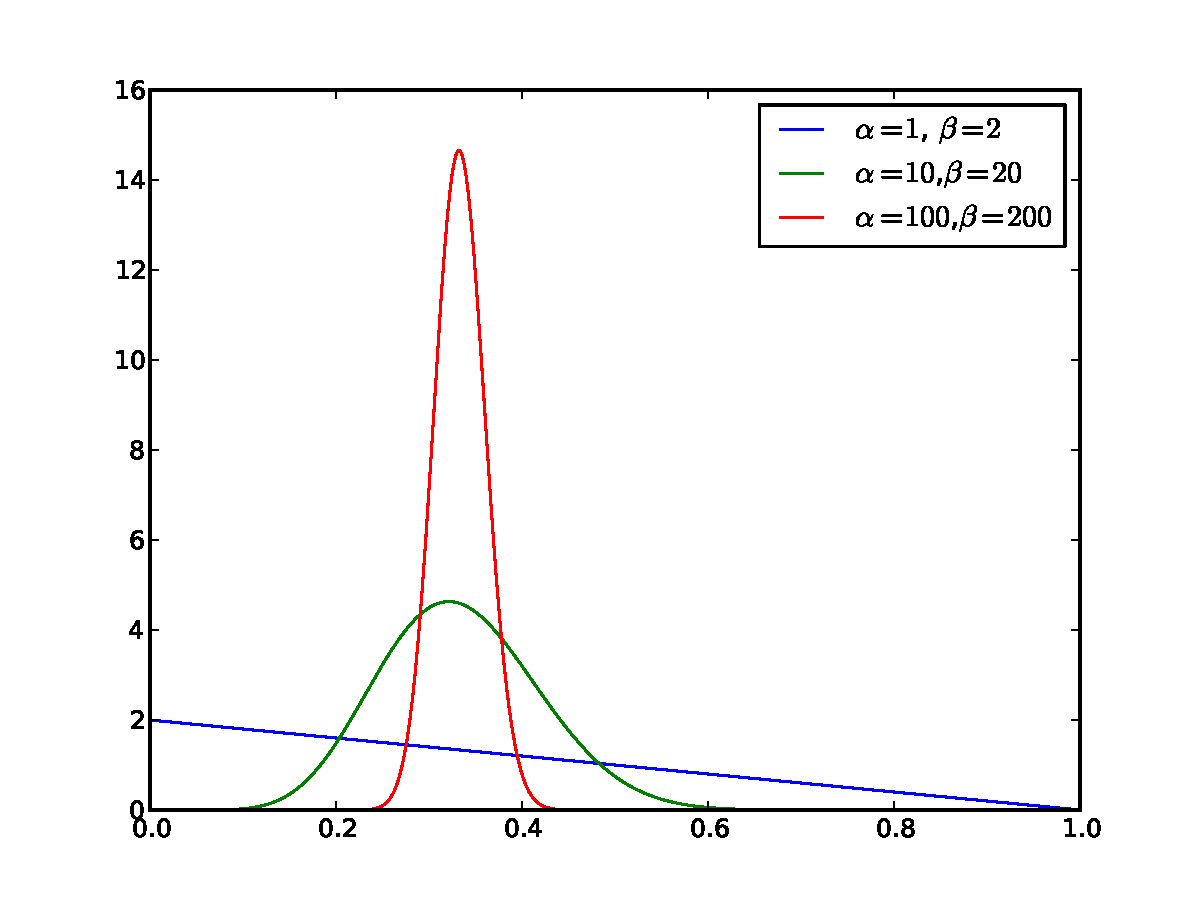
\includegraphics[scale=0.4]{./Algorithms/MarkDecProc/priors.pdf}
        \caption{Bayesian priors}
\end{center}
\end{figure}

The curves are thought of as probability distributions.  So if you have had $1$ success and $2$ failures, you might think that $p_i$ is around $\frac{1}{3} = \frac{1}{1+2}$. However, you have very little information at this point, so better yet you might represent your belief about $p_i$ by the blue probability distribution in Figure \ref{fig:priors}.  We call the distribution that describes our belief about $p_i$ the prior distribution of $p_i$.  If we incorporate new information, we get a new distribution called the posterior distribution.  The posterior distribution can also be thought of as a new prior distribution as we continue to collect information.  

As we get more information, the curve gets narrower.  In the figure, we see that the distributions have expected value of $1/3$ and become tighter around that value.  This is fitting since the parameter values have success $\alpha$ one third of the time and the tighter distributions correspond to having more prior information.  If we need an estimate for $p_i$ we can use the expected value of our distribution corresponding to $p_i$.  We will denote this estimate by $\bar{p_i}$

In this manner we approach the multi-armed bandit problem.  We do not know the $p_i$ but each time we pull an arm, we update our distribution of where we think it might be.  In particular we use a beta distribution to represent our opinion on what the $p_i$ are.  A beta distribution is a continuous probability distribution on the interval $[0,1]$, which corresponds nicely to the possible values of the $p_i$.  Beta distributions have two parameters $a,b$.  So in our problem the state \eqref{state} can be thought of as representing two beta distributions one for each $p_i$. The details of the updating process are unimportant for now, except for this important property: the two parameters $a,b$ correspond exactly with successes and failures.  So if we start with a distribution Beta$(a,b)$ and the next pull is success, our new distribution is Beta$(a+1,b)$ and if the next pull is a failure then the new distribution is Beta$(a,b+1)$.  Notice this corresponds with the way our states evolve.

\section*{Simulation and Sampling in a Bayesian Framework}
Along with the estimate $\bar p_i$, we can also compute many other useful quantities in our Bayesian problem via random sampling.  Essentially, we can take random draws from our prior distribution and estimate the mean, median, or other quantities based on the value of those quantities in the random sample.  This is a very powerful concept that will be explored in more detail in future labs.

\begin{problem}
Write a function sim\_data that accepts an $n\times 2$ array, where each row represents the parameters of a beta distribution, and a positive integer $k$ that represents the number of random draws to return.  The function should return a $k\times n$ matrix where each row has a random sample from each of the $n$ arms.

This can be accomplished with ease using the scipy function scipy.random.beta.
\end{problem}

\begin{problem}
Suppose one of the arms in a bandit problem has the state (or prior distribution of $p_i$) $Beta(100,200)$ corresponding to $100$ successes and $200$ failures.  Simulate 10,000 data points for the distribution $Beta(100,200)$.  Compute $\bar{p_i}$ by finding the mean of the simulated points.  Compute the median.  Also compute the $95$th percentile using the command

\begin{lstlisting}[style = python]
sp.stats.mstats.mquantiles(data,.95)
\end{lstlisting}
where ``data'' is the array containing the 10,000 simulated data points.
\end{problem}

\section*{Direct Dynamic Programming Solution}
This framework lends itself well to a dynamic programming type solutions.  Rather than just letting $R(a_1,b_1,a_2,b_2)$ represent the state, consider it as the value function, meaning the optimal expected value that can be achieved starting from this state.  Then we have

\begin{equation}\label{recurs}
\begin{aligned}
R(a_1,b_1,&a_2,b_2) =\\
 \max&\left\{\bar{p}_1\cdot[1 + \beta R(a_1+1,b_1,a_2,b_2)] + (1-\bar{p}_1)\beta R(a_1,b_1+1,a_2,b_2)\right. ,\\
&  \left.\bar{p}_2\cdot[1 + \beta R(a_1,b_1,a_2+1,b_2)] + (1-\bar{p}_2)\beta R(a_1,b_1,a_2,b_2+1)\right\}
\end{aligned}
\end{equation}

The two terms in the maximization represent the expected value of pulling lever one or lever two respectively.  For example, if lever one is pulled it is expected to yield a reward of 1 with probability $\bar{p_1}$.  We also must account for the expected value of future rewards (discounted by $\beta$) moving to a state with one more success on arm 1.  With probability $1-\bar{p_1}$, lever one does not give a reward and so rewards are simply the discounted expected reward starting in the next state.

Notice that the expressions inside of $R(\cdot)$ on the right side have parameter values that add to one greater than the $R(\cdot)$ on the left side.  So for example if we want to compute $R(1,1,1,1)$ we need to know $R(2,1,1,1)$, $R(1,2,1,1)$, $R(1,1,2,1)$ and $R(1,1,1,2)$ (all possible combinations of parameters that add up to 5).  To compute these, we need to know all possible combinations of parameters that add up to 6, and so on.  Consequently, we could make a guess for all $R$ for all parameter combinations that add up to some large $N$, then work backward until we get to $R(1,1,1,1)$.  This is backward induction, just as we saw in dynamic programming.  However, the number of computations in this problem grow much too quickly because of the branching nature of having multiple arms.  In fact, if there are more than two arms this method of computation is infeasible!


\begin{comment}
\section*{Gittins Index Solution}
One way we might hope to solve a bandit problem is by computing some sort of ``index'' for each arm.  That is, we want a number associated with each arm that in some sense captures the value of pulling that arm.   Ideally such an index would depend only on that arm, and not on the others.  We could then compare the indices for all of the arms and pull the arm with highest index.  It turns out that bandit problems can be solved optimally by such methods and are computationally more feasible than the dynamic programming approach we saw above.

To compute an index for this problem, we consider comparing an arm with unknown payoff probability $p_i$ to an arm with known payoff probability $p$.  Then equation \eqref{recurs} becomes

\begin{equation}\label{index}
\begin{aligned}
R(p,a_i,b_i) = \max&\left\{\frac{p}{1-\beta} \right. ,\\
&  \left.\hat{p}_i\cdot[1 + \beta R(p,a_i+1,b_i)] + (1-\hat{p}_i)\beta R(p, a_i,b_i+1)\right\}.\\
\end{aligned}
\end{equation}

We determine the expected value of pulling the first arm to be $\frac{p}{1-\beta}$ noting that if we pull the deterministic arm once, we will continue pulling it forever as we gain no new information.  In this case the expected reward from pulling the known arm is $p + \beta p + \beta^2 p + \cdots = \frac{p}{1-\beta}$.


If we can find the $p$ such that we are indifferent between the deterministic arm and the unknown arm, this will give us an index that quantifies the value of arm $p_i$ (this can be proved).

Putting all of this together, our algorithm for solving the multi-armed bandit problem with two arms is as follows.  For each arm $i$, compute \eqref{recurs} over a range of $p$ values to find the $p$ such that you would be indifferent between the arm with probability $p$ and arm $i$. Store this as the index $\lambda_i$.  Compare the $\lambda_i$ and pull the arm with largest index.

In order to compute \eqref{index} we use dynamic programming, starting with a guess for $R$ for parameters that add up to some large $N$ and use backward induction.  In the process, we find $R$ and $\lambda_i$ for each combination of parameters that adds up to any $n\leq N$. Thus we do not have to compute new $\lambda_i$ after each pull, we can just look them up.

\section*{Algorithm Outline}
This section will guide you through creating a function that will compute the indices for a given arm.  It will involve writing a number of functions that you can save in the same .py file.

First, we need a function that will compute all the pairs of $a,b$ that add up to some $N$.  We also want the user to be able to input the minimum values of $a$ and $b$ of interest to avoid unnecessary computation.  For example if in practice all of the arms have $a_i \geq 5$ and $b_i \geq 10$, then we are uninterested in smaller $a$, $b$.  The following code accepts the value of $N$ and a minimum value of a and b and returns an $N$ by 2 array with the $a$'s and $b$'s such that $a + b = N$.

\begin{lstlisting}[style = python]

# computes pairs of numbers starting with mina and minb that
# add up to N

def compute_indices(N,mina,minb):
    import scipy as sp
    avec = sp.arange(mina,N-minb+1)
    avec = sp.reshape(avec,(avec.shape[0],1))
    bvec  = sp.arange(N-mina, minb-1,-1)
    bvec = sp.reshape(bvec,(bvec.shape[0],1))
    values = sp.hstack((avec,bvec))

    return values
\end{lstlisting}

In order to perform the backward induction, we need to be able to estimate the value $R(p,a,b)$ for $a+b = N$.  To do so we have to estimate the second quantity in \eqref{index}.  We will estimate it as $(\frac{a}{a+b})/(1-\beta)$.  This is the value one would get by pulling an arm with $p_i$ equal to the expected value of $Beta(a,b)$ forever.
\begin{problem}
Write a function ``end\_reward" that accepts $p,a,b,$ and $\beta$ and returns the estimated value of $R(p,a,b)$ for $a,b$ such that $a+b=N$.
\end{problem}

For convenience it will be nice to have a function that will compute $R(p,a,b)$ given values of $p,\bar{p},a,b,\beta,N$ as well as values of $R(p,a+1,b)$ and $R(p,a,b+1)$.  This should follow directly from \eqref{index}.

\end{comment}

\section*{Thompson Sampling}
There is a method for computing the optimal solution to the multi-armed bandit problem called the Gittins Index Theorem.  Computationally it is similar to the dynamic programming approach, but significantly less costly.  However, for large scale problems it can still be too costly.

There are, however, many heuristic methods of solving the multi-armed bandit problem.  In particular we will use a method sometimes called Thompson Sampling, or Randomized Probability Matching.  The idea is that we should choose arm $i$ with probability equal to the probability that arm $i$ is the best arm.  So if we believe there is an $80\%$ probability that arm 2 is the best arm we will pull it $80\%$ of the time.  The other $20\%$ of the time we would pull arm one which will help give more information about the true value of $p_1$.  In this way we will pull the arms we expect to get the most rewards from most often.  However, we will also pull other arms with some probability so that we accomplish some exploration and gain information on all arms until we are confident we have found the best arm.

\begin{problem}
Write a function that accepts a $k$ by $n$ array of data computed by the function from Problem 1.  

This function should return a vector of the probabilities that each of the $n$ arms is optimal.  This can be computed for each arm by determining in how many of the $k$ simulations that arm had the highest value.  Dividing this number by $k$ will give the proportion of the simulations for which this arm had the greatest probability of success.  This proportion is interpreted as the probability that the arm is the optimal arm.
\end{problem}

In some applications, we might want to run computations once, then pull many arms instead of computing before each pull.  In these cases, rather than compute these probabilities, choose an arm, then recompute, it can be more convenient to view the probabilities as weights.  For example we can view the probabilities as the weights of how to distribute the next 100 pulls.  Suppose the probabilities resulting from the previous function (with two arms) are $0.4$ and $0.6$.  Then we would allot 40 of the next 100 pulls to arm 1 and 60 of the next 100 pulls to arm 2.  Then we could compute new weights for the next 100 pulls.

\begin{problem}
Using the results from the previous problems, write a function that determines how many times each arm should be pulled in the next $M$ pulls where $M$ is an input to the function.  The function should accept a vector of probabilities that of the form returned by the function in the previous problem, and a number of pulls $M$.  Note that you will have to round since the number of pulls for each arm must be in integer.  Return a vector of length $n$ (where $n$ is the number of arms) that gives the number of pulls out of the next $M$ for each arm.  Make sure the entries sum to $M$.
\end{problem}

You now have code that solves the version of the multi-armed bandit problem described here.  To solve such a problem you would first start all arms with the state (or prior) $Beta(1,1)$, which is the uniform distribution, meaning we have no information on the $p_i$.  Then we can compute the weights for the next $M$ pulls.  After those $M$ pulls we can compute new weights and continue on in this pattern.  In some applications we may not continue this forever, but might instead have some stopping criteria for when we think we have identified the best arm.  A common stopping criteria would be to stop when one of the arms has a $95\%$ probability (or some other specified probability) of being the optimal arm.  In the framework we have set up, this is already computed at each step and thus easy to check for.

In the following applications lab, we will investigate how this process can be applied in web page testing and simulate a bandit problem using the functions in this lab.